\documentclass[a4paper, article, oneside, UKenglish]{memoir}


%% Title page
\usepackage{projectfp} % [MAT2000], [MAT2500], [MEK3200] or [STK-MAT2011]


%% Encoding
\usepackage[utf8]{inputenx} % Source code
\usepackage[T1]{fontenc}    % PDF

% \usepackage{natbib} %Bibliography.
% \setcitestyle{number} %Cite as numbers or author-year.
% \bibliographystyle{vancouver} %Reference style.

%% Fonts and typography
\usepackage{lmodern}           % Latin Modern Roman
\usepackage[scaled]{beramono}  % Bera Mono (Bitstream Vera Sans Mono)
\renewcommand{\sfdefault}{phv} % Helvetica
\usepackage[final]{microtype}  % Improved typography
\renewcommand{\abstractnamefont}{\sffamily\bfseries}                 % Abstract
\renewcommand*{\chaptitlefont}{\Large\bfseries\sffamily\raggedright} % Chapter
\setsecheadstyle{\large\bfseries\sffamily\raggedright}               % Section
\setsubsecheadstyle{\large\bfseries\sffamily\raggedright}            % Subsection
\setsubsubsecheadstyle{\normalsize\bfseries\sffamily\raggedright}    % Subsubsection
\setparaheadstyle{\normalsize\bfseries\sffamily\raggedright}         % Paragraph
\setsubparaheadstyle{\normalsize\bfseries\sffamily\raggedright}      % Subparagraph
\usepackage[table]{xcolor}

%% Mathematics
\usepackage{amssymb}   % Extra symbols
\usepackage{amsthm}    % Theorem-like environments
\usepackage{thmtools}  % Theorem-like environments
\usepackage{mathtools} % Fonts and environments for mathematical formuale
\usepackage{mathrsfs}  % Script font with \mathscr{}


%% Miscellaneous
\usepackage{graphicx}  % Tool for images
\graphicspath{{figures/}}
\usepackage{babel}     % Automatic translations
\usepackage{csquotes}  % Quotes
\usepackage{textcomp}  % Extra symbols
\usepackage{listings}  % Typesetting code
\lstset{basicstyle = \ttfamily, frame = tb}
% \usepackage{hyperref}



%% Bibliography
\usepackage{mathscinet}
\usepackage[backend    = biber,
            numbers = true,
            sortcites  = true,
            giveninits = true,
            doi        = false,
            isbn       = false,
            url        = false,
            sortlocale = nb_NO,
            style      = alphabetic]{biblatex}
\DeclareNameAlias{sortname}{family-given}
\DeclareNameAlias{default}{family-given}
\DeclareFieldFormat[article]{volume}{\bibstring{jourvol}\addnbspace#1}
\DeclareFieldFormat[article]{number}{\bibstring{number}\addnbspace#1}
\renewbibmacro*{volume+number+eid}
{
    \printfield{volume}
    \setunit{\addcomma\space}
    \printfield{number}
    \setunit{\addcomma\space}
    \printfield{eid}
}
\addbibresource{bibliography.bib}
\usepackage{url}


%% Cross references
\usepackage{varioref}
\usepackage[pdfusetitle]{hyperref}
\hypersetup{
    colorlinks=true,
    linkcolor=blue,
    filecolor=blue,
    citecolor = blue,      
    urlcolor=cyan,
}
\usepackage{minted}
\urlstyle{sf}
\usepackage[nameinlink, capitalize, noabbrev]{cleveref}
\crefname{chapter}{Section}{Sections}


%% Theorem-like environments
\declaretheorem[style = plain, numberwithin = chapter]{theorem}
\declaretheorem[style = plain,      sibling = theorem]{corollary}
\declaretheorem[style = plain,      sibling = theorem]{lemma}
\declaretheorem[style = plain,      sibling = theorem]{proposition}
\declaretheorem[style = definition, sibling = theorem]{definition}
\declaretheorem[style = definition, sibling = theorem]{example}
\declaretheorem[style = remark,    numbered = no]{remark}


%% Delimiters
\DeclarePairedDelimiter{\p}{\lparen}{\rparen}   % Parenthesis
\DeclarePairedDelimiter{\set}{\lbrace}{\rbrace} % Set
\DeclarePairedDelimiter{\abs}{\lvert}{\rvert}   % Absolute value
\DeclarePairedDelimiter{\norm}{\lVert}{\rVert}  % Norm


%% Operators
\newcommand{\diff}{\mathop{}\!\mathrm{d}}
\DeclareMathOperator{\im}{im}
\DeclareMathOperator{\rank}{rank}
\DeclareMathOperator{\E}{E}
\DeclareMathOperator{\Var}{Var}
\DeclareMathOperator{\Cov}{Cov}


%% New commands for sets
\newcommand{\N}{\mathbb{N}}   % Natural numbers
\newcommand{\Z}{\mathbb{Z}}   % Integers
\newcommand{\Q}{\mathbb{Q}}   % Rational numbers
\newcommand{\R}{\mathbb{R}}   % Real numbers
\newcommand{\C}{\mathbb{C}}   % Complex numbers
\newcommand{\A}{\mathbb{A}}   % Affine space
\renewcommand{\P}{\mathbb{P}} % Projective space


%% New commands for vectors
\renewcommand{\a}{\mathbf{a}}
\renewcommand{\b}{\mathbf{b}}
\renewcommand{\c}{\mathbf{c}}
\renewcommand{\v}{\mathbf{v}}
\newcommand{\w}{\mathbf{w}}
\newcommand{\x}{\mathbf{x}}
\newcommand{\y}{\mathbf{y}}
\newcommand{\z}{\mathbf{z}}
\newcommand{\0}{\mathbf{0}}
\newcommand{\1}{\mathbf{1}}


%% Miscellaneous
\renewcommand{\qedsymbol}{\(\blacksquare\)}


\title{Data Modeling Project}
\author{Sai Nikhil Thirandas}
\supervisor{Prof. Christopher King}
% Multiple supervisors: \supervisor{Supervisor 1}{Supervisor 2}...{Supervisor n}
% Skip supervisor for MAT2500


\begin{document}


\projectfrontpage


% \begin{abstract}
%     \noindent
%     Brief summary of the paper.
% \end{abstract}



\chapter{Description of Data}

I downloaded a compilation of historical baseball data from Kaggle - Baseball Databank \cite{BD}. The data is contributed by Sean Lahman \cite{BDB}. It contains batting statistics such as playerID, year, stint (order of appearance), teamID, Runs Scored by Player in Match, etc., at the international league level. There are in total 101333 rows, each corresponding to a unique combination of player and year between years 1871 and 2015 (boundaries included). For example we can have data of 200 players with corresponding stints in 1871 and 180 players with corresponding stints in 1872 etc., There can be some overlap in players year to year or may not. Because a player can retire after a certain age limit is reached.

\chapter{Cleaning of Data}

I picked only those rows for the first stint (opening batsman) and took an average of runs scored by all the players appearing at stint 1 in each year. So my new data will look something like a combination of years and runs, where years will correspond to index of time series and runs are average of all opening players (stint = 1). This can be achieved using a pivot table indexed on year and using the aggregate function as average, applied of runs for which stint = 1. Although the data will just consist of only 145 rows (with rows one each for years from 1871 to 2015) it is formed from a data of 93898 rows (not 101333 because I choose only stint = 1. It is expected to have many entries for stint = 1 because every match is definitely supposed to have opening batsmen). So, on average we are having $\frac{93898}{145} \approx 647$ opening appearances every year which is directly proportional to the number of matches. The reason for choosing the data in the format year vs average of runs is because each year we can have different number of matches played. For example, here in the year 1871, 115 matches were played, in year 1872, 143 matches were played, in year 2012, 1284 matches were played etc., One can clearly observe there is a stark contrast in the number of matches taking place each year. Hence, it is necessary to use some statistical analysis and choose the right central tendency measurement in order to compare data between years. In this case, my personal interest is to compare the average of runs scored by all opening stint players across all the years. So, the time series plot of years vs average runs of opening batsman would look like the below graph:


\centerline{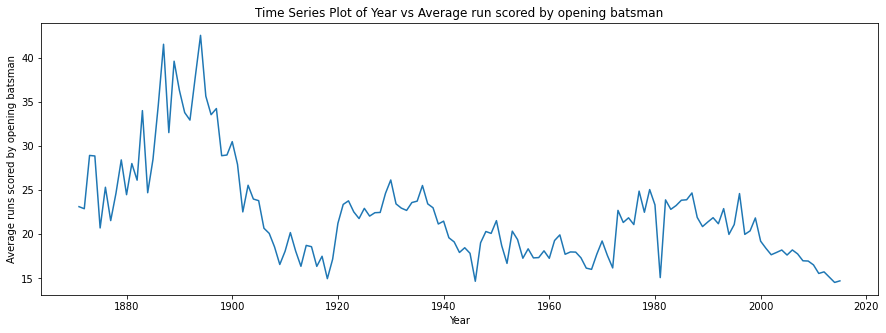
\includegraphics[scale=0.5]{projectfp-images/YearVsAverageRunsPlot.png}}


\chapter{Data Analysis \& Modeling}

From the above graph, I observed that there are several outliers. For example, During 1890 - 1900, the average runs scored by opening batsman is very high. I first tried diving the range of average runs into equal intervals and found that my modelling is behaving poorly for all the states. I realized that is not a fair assumption to divide the intervals of the range of average runs into equal lengths. Hence, upon having a close look at the data I found that diving the values such that each state follows the following distribution is a fair assumption.

\begin{minted}{python}
quantiles = [0.03, 0.24, 0.52, 0.69, 0.83, 0.935, 0.97, 0.99, 1.0]
\end{minted}

The total number of states in the Markov Chain are 9. This produces a left skewed curve with median lying at the third state. This looks like a fair assumption because if we closely observe the average run values it is less in the recent days. So the time series frequency plot of Markov State vs the Normalized Frequency should be designed in such a way that median values are closer to least numbered Markov State as it would allow less number of intervals (hence more gap occupied) below the median thus allowing the future value to choose a Markov State of smaller number with higher probability than a Markov State of larger number. According to the above theory, the Markov State vs Normalized Frequency Plot would look like the below graph:

\centerline{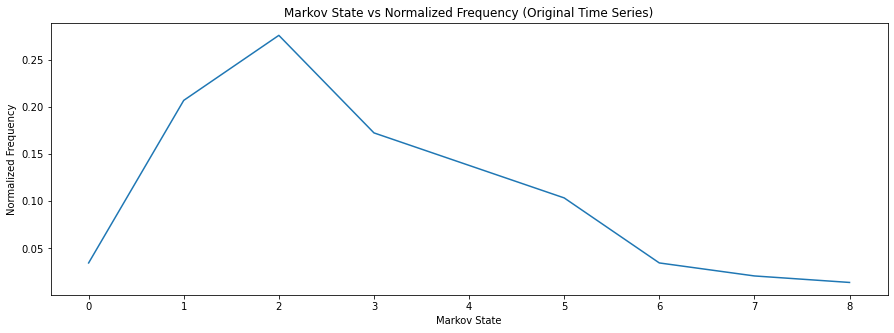
\includegraphics[scale=0.5]{projectfp-images/MarkovStateVsNormalizedFrequencyPlotOriginal.png}}

\section{Empirical Distribution}
The empirical distribution of time series is a plot of time vs Markov State, which would look like the below graph:

\centerline{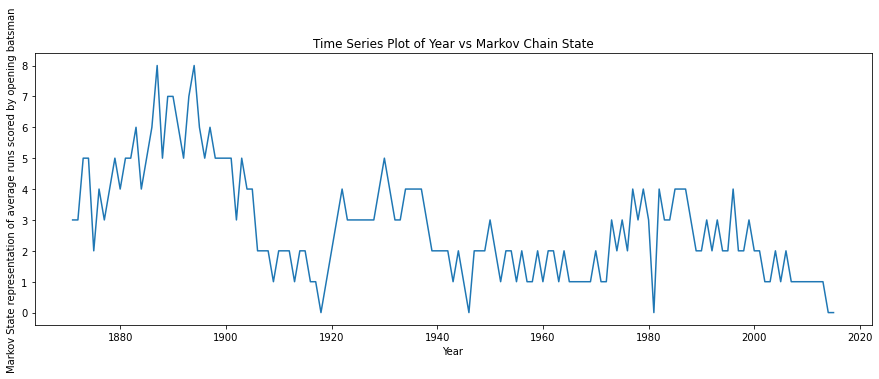
\includegraphics[scale=0.5]{projectfp-images/YearVsMarkovStateOriginal.png}}

\section{Transition Matrix}
I wrote a function in order to \hyperref[sec:tm]{compute the transition matrix} for the time series which follows the above distribution. The transition matrix looks like following:

\begin{minted}[float,caption={Transition Matrix},xleftmargin=-.15\textwidth]{python}
   0.250    0.250    0.250    0.000    0.250    0.000    0.000    0.000    0.000 
   0.100    0.467    0.400    0.033    0.000    0.000    0.000    0.000    0.000 
   0.000    0.375    0.400    0.150    0.075    0.000    0.000    0.000    0.000 
   0.040    0.000    0.320    0.320    0.240    0.080    0.000    0.000    0.000 
   0.000    0.000    0.100    0.400    0.300    0.200    0.000    0.000    0.000 
   0.000    0.000    0.067    0.067    0.200    0.333    0.200    0.133    0.000 
   0.000    0.000    0.000    0.000    0.200    0.600    0.000    0.000    0.200 
   0.000    0.000    0.000    0.000    0.000    0.000    0.333    0.333    0.333 
   0.000    0.000    0.000    0.000    0.000    0.500    0.500    0.000    0.000
\end{minted}

\section{Stationary Distribution}
I wrote a function to \hyperref[sec:sv]{compute the limiting probability vector} (stationary vector) for the empirical distribution. The stationary vector looks like the following:

\begin{minted}[float,caption={Transition Matrix},xleftmargin=-.07\textwidth]{python}
   W = [0.037, 0.214, 0.279, 0.163, 0.138, 0.101, 0.034, 0.020, 0.014]
\end{minted}

As a side note, the above vector is an approximate answer. Because, the system is inconsistent after adding an additional condition, which is sum of $w_i = 1$. It is computed using least squares approximation numerical computation technique.

The Markov State vs stationary vector plot would look like the following graph:

\centerline{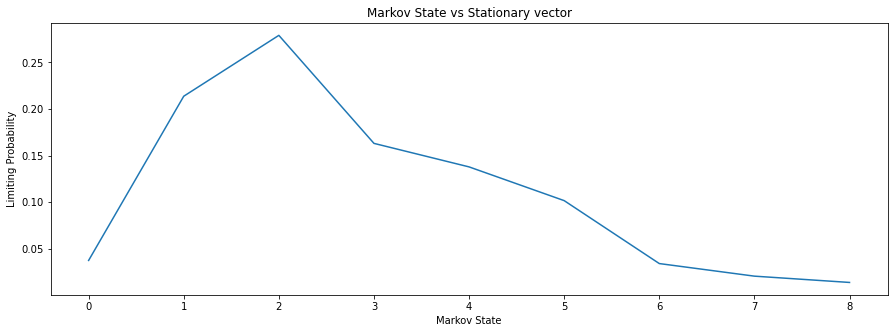
\includegraphics[scale=0.5]{projectfp-images/MarkovStateVsStationaryVectorPlot.png}}

This plot is clearly similar to the Markov State vs Normalized Frequency for original time series which is a indication that I didn't disturb the frequency distribution of the original data.

\section{Simulated Time Series Generation}
I generated a new time series from the stationary vector in the following way. I choose a random seed from state = 0 to state = 8 (my highest Markov state id, because total states = 9 and initial state id = 0). I generate my next state by following a probability distribution as obtained from the transition matrix computed above. For example, if my first random state is, state = 2, then I go to third row in the transition matrix, pick the probability vector (elements in that row) and generate my second state based on this probability vector. If I get my second state as, state = 4, then I go to fourth row in transition matrix, pick the probability vector and generate my third state based on this probability vector and so on ... till I get 145 observations. This is my new time series. As a comparison, the original time series is compared with this simulated time series as a plot and it looks like the following graph:


\centerline{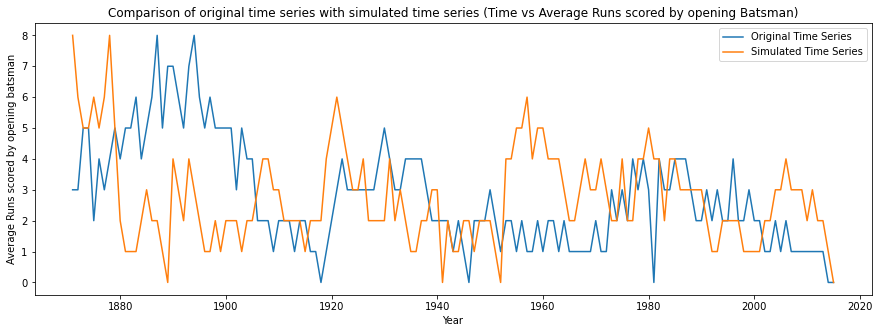
\includegraphics[scale=0.5]{projectfp-images/OriginalTSVsSimulatedTS.png}}

\section{Auto-Correlation Comparison}
Applying the \hyperref[sec:ac]{auto correlation} formula, the correlation values for original time series and simulated time series are given in the following table:

\setlength{\arrayrulewidth}{1mm}
\setlength{\tabcolsep}{18pt}
\renewcommand{\arraystretch}{2.5}

{\rowcolors{3}{gray!30}{gray!15}
\begin{tabular}{ |p{1cm}|p{3cm}|p{3cm}|  }
\hline
\multicolumn{3}{|c|}{Auto correlation values (R)} \\
\hline
k& For Original Time Series& For Simulated Time Series\\
\hline
0 & 1.01899782 &  1.02371143\\
1 & 0.7960541  &  0.67928436\\
2 & 0.74913512 &  0.47582175\\
3 & 0.73698871 &  0.35648656\\
4 & 0.67902765 &  0.21534056\\
5 & 0.65139905 &  0.13500697\\
6 & 0.60837141 &  0.11537835\\
7 & 0.58751107 &  0.0911297 \\
8 & 0.52760434 & -0.03744554\\
9 & 0.46964328 & -0.11079537\\
\hline
\end{tabular}
}

\vspace{10px}

The observation is that values of Zeroth and First auto correlation values of original time series vs simulated time series are very close. The percentage of difference increases as we go down the table. This is in general not a good sign and can lead to a conclusion that our original time series is not a Markov Chain. Further analysis is needed which is done below.
\section{Goodness of Fit Test}
A Goodness of Fit Test for two step transition of original time series is conducted in order to see if our original time series obeys Markov Principle (current state is dependent only on previous state and not anything before that). The Pearson Test Statistic values are computed for each state and this value is compared with chi-squared probability density function with corresponding degrees of freedom obtained from empirical distribution with two step transition where the entry is greater than zero in theoretical distribution and 5 percent significance level, using the function \hyperref[sec:tscs]{compute\_test\_statistic}. This comparison yielded following results:


\setlength{\arrayrulewidth}{1mm}
\setlength{\tabcolsep}{18pt}
\renewcommand{\arraystretch}{2.5}

{\rowcolors{3}{grey!20}{grey!10}
\begin{tabular}{ |p{0.3cm}|p{2.5cm}|p{2.5cm}|p{1.5cm}|  }
\hline
\multicolumn{4}{|c|}{Comparison of Chi-square with Test Statistic for each state} \\
\hline
State& Chi Square Value & Test Statistic & Decision\\
\hline
0 & 7.814727903251179  & 28.5                   & Rejecting\\
1 & 7.814727903251179  & 157.7253401360544       & Rejecting\\
2 & 7.814727903251179  & 70.21227564102563       & Rejecting\\
3 & 9.487729036781154  & 141.50464629629627       & Rejecting\\
4 & 7.814727903251179  & 148.60524691358023       & Rejecting\\
5 & 11.070497693516351 &  104.23495726495725      & Rejecting\\
6 & 5.991464547107979  &  3.6533333333333333       & Accepting\\
7 & 5.991464547107979  &  14.666666666666664       & Rejecting\\
8 & 3.841458820694124  &  2.5                   & Accepting\\

\hline
\end{tabular}
}

\vspace{10px}

\chapter{Conclusions}

This comparison shows that GoF test rejected the states 0, 1, 2, 3, 4, 5, 7 and accepted states 6, 8. This is another confirmation (apart from auto-correlation test) that this time series does not obey the Markov Rule (current state is dependent only on previous state and not anything before that).

So our initial assumption that the average of runs scored by opening batsman is just dependent on the average of runs scored by opening batsman only in previous year is wrong. It could be true because in practice this is a multidimensional problem which can depend on several features and we tried to simplify the model with an assumption that it follows Markov Rule (current state is dependent only on previous state and not anything before that). In fact, batsman change every year and number of matches played differ every year and if in a year the strong team plays more number of matches, the average runs scored by opening batsman could be more and if weaker teams play more number of matches in a certain year, the average runs scored by opening batsman could be less etc., However, this analysis is still very useful because if it works out well, our model is greatly simplified and if it doesn't work well then we can conclude to not use Markov Modeling for this problem statement in the future.


\chapter{Appendix}

\section{Function to compute transition matrix}
\label{sec:tm}
\begin{minted}{python}
def compute_transition_matrix_fast(data, n, step = 1):
    t = np.array(data)
    step = step
    total_inds = t.size - (step + 1) + 1
    t_strided = np.lib.stride_tricks.as_strided(
                                    t,
                                    shape = (total_inds, 2),
                                    strides = (t.strides[0], step * t.strides[0]))
    
    inds, counts = np.unique(t_strided, axis = 0, return_counts = True)

    P = np.zeros((n, n))
    N = np.zeros((n, n))
    P[inds[:, 0], inds[:, 1]] = counts
    N[inds[:, 0], inds[:, 1]] = counts
    
    sums = P.sum(axis = 1)
    
    P[sums != 0] = P[sums != 0] / sums[sums != 0][:, None]
    
    return P, N
\end{minted}

\section{Function to compute Stationary Vector}
\label{sec:sv}
\begin{minted}{python}
def compute_stationary_distribution(P):
    A = np.vstack((P.T - np.identity(P.shape[0]), np.ones((P.shape[0]))))
    # print(A.shape)
    b = np.zeros((P.shape[0] + 1, 1))
    # print(b.shape)
    # print(b)
    b[-1] = 1
    # print(b)
    # display(sp.Matrix(A))
    return np.linalg.lstsq(A, b)[0]
\end{minted}

\section{Function to compute Auto Correlation}
\label{sec:ac}
\begin{minted}{python}
def compute_auto_correlation(x, k):
    x_bar = np.average(x)
    num, den = 0, 0
    m, M = x.index.min(), x.index.max()
    
    for i in range(m, M - k + 1):
        num += ((x[i] - x_bar) * (x[i + k] - x_bar))
    
    for i in range(m, M):
        den += (x[i] - x_bar)**2
    
    return num / den
\end{minted}

\section{Function to compute test statistic and chi square value for each state}
\label{sec:tscs}
\begin{minted}{python}
def compute_test_statistic(N, Q, i):
    n, N2 = N.shape[0], N[i][Q[i] > 0]
    S = N2.sum()
    chi2 = sc.stats.chi2.ppf(q = 0.95, df = len(N2) - 1)
    ts = 0.0
    # print(n, S)
    if S > 0:
        for j in range(n):
            if Q[i][j] > 0:
                observed = N[i][j]
                expected = S * Q[i][j]
                ts += ((observed - expected)**2 / expected)
    return chi2, ts
\end{minted}


\printbibliography

\end{document}